
\documentclass[aps,prstab,twocolumn,superscriptaddress,groupedaddress,showkeys,nofootinbib]{revtex4}  % for review and submission
%\documentclass[aps,preprint,showpacs,superscriptaddress,groupedaddress]{revtex4}  % for double-spaced preprint
\usepackage{graphicx}  % needed for figures
\usepackage{dcolumn}   % needed for some tables
\usepackage{bm}        % for math
\usepackage{amssymb}   % for math
\usepackage{graphicx,subfigure}
\usepackage[]{mcode}

% avoids incorrect hyphenation, added Nov/08 by SSR
\hyphenation{ALPGEN}
\hyphenation{EVTGEN}
\hyphenation{PYTHIA}

\begin{document}

\widetext

\leftline{Computational Electromagnetics (EE640) Term Paper, April 2014 }

\title[Computational Electromagnetics (EE640) Term Paper]{Analysis of linear wire antenna using Method of Moment (MoM)}
\author{Kapil Saraswat\\PhD Scholar\\Roll No. 13104176\\ \textbf{Instructor:} Dr. A.R. Harish}
\date{\today}
\begin{abstract}

\textbf{\textit{Abstract}}\\
In this Term paper submission, rigorous analysis of linear thin wire using method of moment is presented. The current distribution and input impedance of linear wire antenna are reviewed. The effect of different basis function eg. entire domain and sub domain basis function are discussed. In the analysis of linear wire, Pocklington's and Hallen's integral equation is employed. The effect of discretization are studied. The convergence of input impedance for different source models are studied. 
\end{abstract}
\keywords{Method of Moment, linear wire antenna, entire domain basis function, sub-domain basis function, Pocklington,s integral equation, Hallen's integral equations }


\maketitle

\section{Introduction}
The electromagnetic  problems can be categorized in three different ways 1.) Using solution region of the electromagnetic problem 2.) The problem described by the mathematical equation 3.) Using boundary conditions incorporated with the problem domain\cite{sadiku}.The electromagnetic problem described by the equation could be integral, differential or integro-differential equation and can be defined in terms of operator equation \cite{sadiku}.\\
The differential equation is usually simpler and approach to the exact solution of the given problem. The integral equation approach to approximate solution and the boundary conditions are imposed to the integral equation \cite{garg}. In general, the differential equations are solved using Finite Element Method (FEM) while the integral equations are solved using Method of Moment. The Method of Moment (MoM) is a numerical technique to reduce an operator equation ( like integral, differential or integro-differential equation) to matrix equation \cite{harri}.\\
This term paper begins with the Method of Moment for the solution of deterministic problem. Then the Pocklington's equation and Hallen's equation are formulated for the wire antenna. The solution to Pocklington's and Hallen's equation, using method of moment, is then explained. The integral equation solution using MoM yields the current distribution on the wire. Using the surface current distribution on the antenna other antenna parameters ( like gain, input impedance, directivity etc) can be easily computed.\\
Further, the entire domain and sub-domain basis functions are compared using the surface current distribution on wire antenna. The effect of  segmentation (or discretization) on solutions are demonstrated.
\section{Method of Moment}
Consider the homogeneous equation\cite{harri}
\begin{equation}
L\left ( \mathit{f} \right )=g
\end{equation}
where L is a linear operator, g is known excitation function and \textit{f} is to be determined. Let \textit{f} be expanded in a sum of basis functions, $f_{n}$, as
\begin{equation}
\mathit{f}=\sum_{n}\alpha_{n} \mathit{f}_{n}
\end{equation}
A set of equations for the coefficients $\alpha_{n}$ are then obtained by taking the inner product of equation (1) with a set of weighting functions {$w_{m}$},
\begin{eqnarray}
<w_{m},L\mathit{f}>= <w_{m},L(\mathit{e})> \\ \nonumber
i=1,2,3,...n
\end{eqnarray}
Due to the linearity of L equation (2) substituted for \textit{f} yields
\begin{eqnarray}
\sum_{n}\alpha_{n}<w_{m},L\mathit{f_{n}}>= <w_{m},\mathit{e}> \\ \nonumber
i=1,2,3,...n
\end{eqnarray}
This equation can be written in matrix notation as,
\begin{equation}
\left [ G_{mn} \right ]\left [A_{n}  \right ]=\left [ E_{m} \right ]
\end{equation}
where,\\
\begin{center}
$G_{mn}=<w_{m},L\textit{f}_{n}>$\\
$A_{n}=\alpha_{n}$ \\
$E_{m}=<w_{m},\textit{e}>$\\
\end{center}
If the matrix [G] is nonsingular, its inverse exists and the solution ( unknown coefficient) is 
\begin{equation}
\left [ A \right ]=\left [G  \right ]^{-1}\left [ E \right ]
\end{equation}
and 
\begin{equation}
\mathit{f}=[f_{n}][\alpha_n]=[f_{n}][G_{mn}]^{-1}[E]
\end{equation}
Depending upon the choice of the $\textit{f}_{n}$ and  $w_{m}$ the solution may be exact or approximate. In special case when, $\textit{f}_{n}= w_{m}$  it is known as Galerkin's method.
\section{Thin Wire}
Present term paper is focused to the moment analysis of linear wire antennas using Pocklington's and Hallen's equation. Throughout this paper, the linear wire antenna is supposed to be cylindrical in shape with radius \textit{a} and length 2\textit{l}. Figure 1 shows the geometry of wire antenna from which Pocklington's and Hallen's integral equation can be derived. Pocklington's integro-differential equation and Hallen's integral equation are widely used to find the current distribution on conducting thin wires \cite{sadiku}. Hallen's equation is restricted to the use of delta-gap excitation (see \textbf{Appendix A}). Pocklington's equation is more general and it is adaptable to many types of feed sources (see \textbf{Appendix A}).
\begin{figure}[here!]
\centering
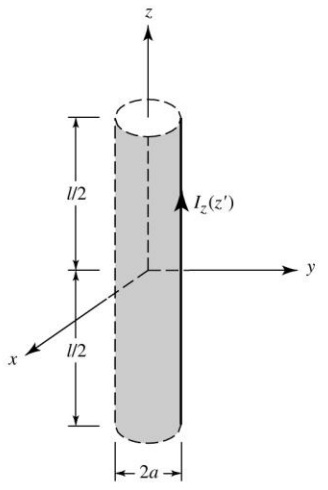
\includegraphics[scale=0.5]{image1.jpg}
\caption{Geometry of wire for integral equation formulation}
\end{figure}
\subsection{Pocklington's Equation}
A well known formulation for linear wire antennas is Pocklington's integro-differential equation. Let the antenna (along z-direction) be situated in a lossless homogeneous dielectric medium ($\sigma=0$). Assuming a z-directed current on the cylinder ($\textbf{J}=J_{z}a_{z}$), due to axial symmetry only $E_{z}$ is produced. In terms of retarded potential, the electric field can be expressed as,
\begin{equation}
E_{z}=-j \omega A_{z}-\frac{\partial V}{\partial z}
\end{equation}
Applying the lorentz condition i.e.
\begin{equation}
\frac{\partial A_{z}}{\partial z}=-j \omega \mu \epsilon V
\end{equation}
Equation 8 becomes
\begin{equation}
E_{z}=-j \omega \left (1+\frac{1}{k^{2}}\frac{\partial^2 }{\partial z^2} \right )A_{z}
\end{equation}
where the wave number, k, defined as $ k=\omega (\mu \epsilon )^{\frac{1}{2}}=\frac{2\pi }{\lambda }$ , $\omega$ is the angular frequency of the suppressed harmonics time variation $e^{j\omega t}$. Using Electric Field Integral Equation (EFIE) and and neglecting edge effects, 
\begin{equation}
A_{z}=\mu \int_{-l/2}^{l/2}I(z')G(x,y,z:x',y',z')dz'
\end{equation}
where G(x,y,z:x',y',z') is the free space green's function defined as,
\begin{equation}
G(x,y,z:x',y',z')=\frac{e^{-jkR}}{4 \pi R}
\end{equation}
and R is the distance between observation point (x, y, z) and source point (x', y', z') or 
\begin{equation}
R=\sqrt{(x-x')^{2}+(y-y')^{2}+(z-z')^{2}}
\end{equation}
From equation (10) and (11) we get,
\begin{equation}
E_{z}=-j \omega \mu \left (1+\frac{1}{k^{2}}\frac{\partial^2 }{\partial z^2} \right ) \int_{-l/2}^{l/2}I(z')G(x,y,z:x',y',z')dz'
\end{equation}
Introducing operator inside the integral sign and multiply with $j\omega \epsilon $ we get,
\begin{equation}
j \omega \epsilon E_{z}= \int_{-l/2}^{l/2}I(z')\left (k^{2}+\frac{\partial^2 }{\partial z^2} \right )G(z:z')dz'
\end{equation}
For very thin wire $ (a<< \lambda) $, equation(15) can be written as,
\begin{equation}
j \omega \epsilon E_{z}= \int_{-l/2}^{l/2}I_{z}(z')\frac{e^{-jkR}}{4 \pi R^{5}}\left [ (1+jkR)(2R^2-3a^2)+(kaR)^2 \right ]dz'
\end{equation}
Equation 15 is known as Pocklington's integral Equation. The Pocklington's integral equation can be used to determine the equivalent line current of the wire, and thus current density on the wire, by knowing the incident field on the surface of antenna.
\subsection{Hallen's Integral Equation}
For wire antenna $(a<<\lambda)$ neglecting the the effect of end faces, the boundary condition for a wire with infinite conductivity are those of vanishing total tangential $\vec{E}$ fields on the conducting surface of the wire. This vanishing the currents at the ends of the cylinder [$I_{z}(z'=\pm l/2)=0$]. Since it is z-directed, $ (\vec{J}=\hat{a}_{z}J_{z})$ therefore \cite{bala},
\begin{equation}
\vec{A}=\hat{a}_{z}A_{z}(z')
\end{equation}
and 
\begin{equation}
E^{t}_{z}=-j \omega A{z}-\frac{j}{\omega \mu \epsilon}\frac{\partial^2 A_{z}}{\partial z^2}
\end{equation}
or
\begin{equation}
E^{t}_{z}=\frac{-j}{\omega \mu \epsilon}\left [ \frac{\partial^2 A_{z}}{\partial z^2}+\omega ^{2} \mu \epsilon A_{z} \right ]
\end{equation}
Since the total tangential electric field $E^{t}_{z}$ vanishes on the surface of the cylinder therefore,
\begin{equation}
\frac{\partial^2 A_{z}}{\partial z^2}+k^{2} A_{z}=0
\end{equation}
$\because J_{z}(z')=J_{z}(-z')$, symmetrical current density hence the potential $A_{z}$ is also symmetrical i.e. $ A_{z}(z')=A_{z}(-z')$. Thus the solution of equation (20) is given by,
\begin{equation}
A_{z}(z)=-j \sqrt{\mu \epsilon}\left [ B_{1}cos(\beta z)+C_{1}sin(\beta \left |z  \right |) \right ]
\end{equation}
Where $B_{1}$ and $C_{1}$ are constants. Equating equation (11) and 20 leads to,
\begin{equation}
\int_{-l/2}^{l/2}I(z')\frac{e^{-j \beta R }}{4 \pi R} dz'=-j \sqrt{\frac{\epsilon}{\mu}}\left [ B_{1}cos(\beta z)+C_{1}sin(\beta \left |z  \right |) \right ]
\end{equation}
For input voltage $V_{i}$ at the input terminal of the wire, the constant can be given as $c_{1}=\frac{v_{i}}{2}$. The constant $B_{i}$is determined from the boundary condition \cite{class}. Equation (22) is known as Hallen's Integral Equation. 
\subsection{Formulation of Method of Moment for wire antenna }
In Method of Moment, orthogonal expansions and linear algebra are used to reduce linear deterministic problem \cite{paper1}. The procedure for applying Method of Moment to solve Pocklington's or Hallen's integral equation usually involves following steps \cite{sadiku}:
\begin{enumerate}
\item Derivation of the integral equation, in our case Pocklington's or Hallen's Integral Equation.
\item Discretization of the integral equation into a matrix equation employing Basis functions and Weighting functions. (see \textbf{Appendix B} for Basis and Weighting function)
\item Evaluation of the matrix elements and
\item Obtaining unknown coefficients (or parameters) by  Solving the matrix.
\end{enumerate}
After formulating the deterministic EM problem in terms of Pocklington's or Hallen's integral equations, we can transform integral equation into matrix form using MoM. As discussed above, after defining IE problem, discretized the wire uniformly to N equal segments.Applying the point matching technique (or galerkin's approach), take observation(field) points (or matching points) $Z_{m}$ at the midpoint of each subinterval as shown in Figure 2 where the positions of $Z_{m}$ and $Z_{n}$ are 
\begin{equation}
z_{m}=\frac{(2m-1)l}{2N}; m=1,2,3,...N+1 \\ 
\ z_{n}=\frac{(n-1)l}{N}
\end{equation}
Now approximate $I(z)$ as 
\begin{eqnarray}
P_{n}(z)= 1 &&  z_{n} \in \triangle z \\ \nonumber 
0 && z_{n} \notin \triangle z 
\end{eqnarray}
Substitute these values in equation (16) or (22), we get 
\begin{equation}
\left [ G_{mn} \right ]\left [A_{n}  \right ]=\left [ E_{m} \right ]
\end{equation}
%Therefore the matrix equation is in the form,
%\[ \begin{vmatrix}
% G_{11}&   G_{12}& ... &  G_{1N} & \\ 
% G_{21}&   G_{22}& ... &  G_{2N} & \\ 
% G_{31}&   G_{32}& ... &  G_{3N} & \\ 
% G_{41}&   G_{42}& ... &  G_{4N} & \\ 
% G_{N1}&   G_{N2}& ... &  G_{NN} & \\ 
%\end{vmatrix}\begin{vmatrix}
% A_{1}&\\ 
% A_{2}&\\
% A_{3}&\\ 
% A_{4}&\\ 
% A_{N}&\\ 
%\end{vmatrix}=\begin{vmatrix}
% E_{1}&\\ 
% E_{2}&\\
% E_{3}&\\
% E_{4}&\\
% E_{N}&\\
%\end{vmatrix}\] 
\begin{figure}[here!]
\centering
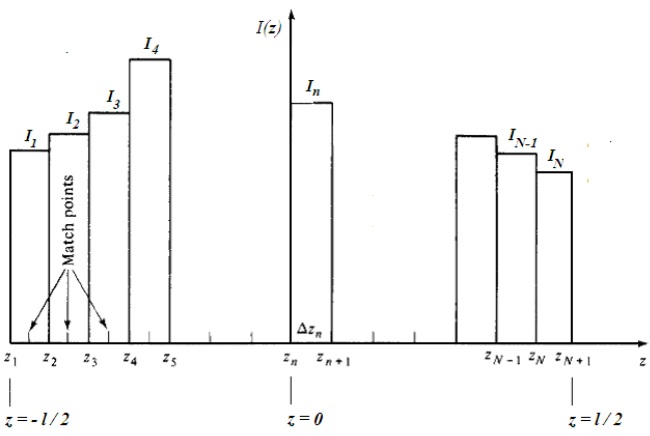
\includegraphics[scale=0.45]{image2.jpg}
\caption{Discretization of wire antenna}
\end{figure}
In next section, the implementation of Pocklington's and Hallen's Integral Equation in MATLAB is discussed. The effect of source modeling is discussed in Appendix A. 
\vspace{-5mm}
\subsubsection{Pocklington's Integral Equation}
In the matlab equation (16) is implemented for Pocklington's integral equation for thin wire antenna. The MATLAB code is as follows
\begin{lstlisting}
        if (n==N+1)
            A(m,n)=-i*cos(k*zm)/(etha);
        else
            syms z
            R=sqrt(a^2+(z-zm)^2);
            g=inline([exp(-i*k*R)/(4*pi*R^5)]*[(1+j*k*R)...
                 *(2*R^2-3*a^2)+(k*a*R)^2]);
            G=quad(g,zn,zn+delta);
            A(m,n)=-lamda*etha*G/(8*pi^2*i);
        end
\end{lstlisting}
Where the inline function represents the Pocklington's equation, and the MATLAB command quad tries to approximate the integral of scalar-valued function within an error of 1.e-6 using recursive adaptive Simpson quadrature \cite{matlab}.
\vspace{-5mm}
\subsubsection{Hallen's Integral Equation}
In the matlab equation (22) is implemented for Hallen's integral equation for thin wire antenna. The MATLAB code is as follows
\begin{lstlisting}
        if (n==N+1)
            A(m,n)=-cos(k*zm);
        else
            syms z
            R=sqrt(a^2+(z-zm)^2);
            g=inline([exp(-i*k*R)/(4*pi*R)]);
            G=quad(g,zn,zn+delta/2);
            A(m,n)=G;
        end
\end{lstlisting}
Where the inline function represents the Hallen's integral equation (L.H.S.) , and the MATLAB command quad tries to approximate the integral of scalar-valued function within an error of 1.e-6 using recursive adaptive Simpson quadrature \cite{matlab}.\\
At the end, impedance matrix is inverted and its respective column gives the values of the current distribution. 
\begin{lstlisting}
	V(m,1)=[-i*Voltage*sin(k*abs(zm))]/(2*etha);
	Ainv=inv(A);
	% Surface current distribution
	I=(Ainv*V);
	% input Impedance
	Zinp = 1.0 / I(floor(N/2)+1)
\end{lstlisting}
\section{Result}
Figure 3 Shows the surface current distribution on the linear dipole antenna using Pocklington's integral equation for point matching MoM. The frequency of operation is 300 Mhz, length of dipole is $\frac{\lambda }{2}$, diameter of wire is $\frac{\lambda }{500}$ and N=51.\\
Total simulation time is 249.345 sec. During the simulation the maximum time was consumed by function name sym.sys which is used for the symbolic manipulation in the integral equation. quad function was called 3932 times with total time 25.722 sec in single simulation. 
\begin{figure}[here!]
\centering
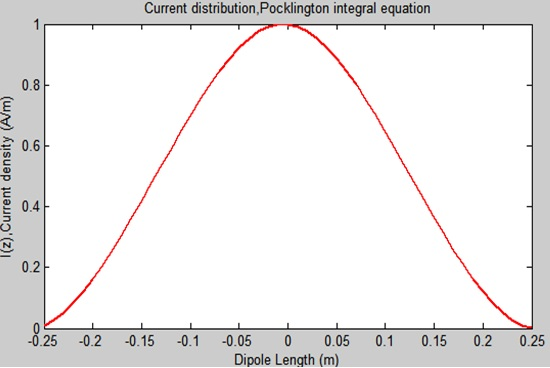
\includegraphics[scale=0.5]{image3.jpg}
\caption{Pocklington's Integral Equations; Current distribution on the wire antenna with f=300MHz, L=$\frac{\lambda }{2}$, 2a=$\frac{\lambda }{500}$ and N=51}
\end{figure}
\begin{figure}[here!]
\centering
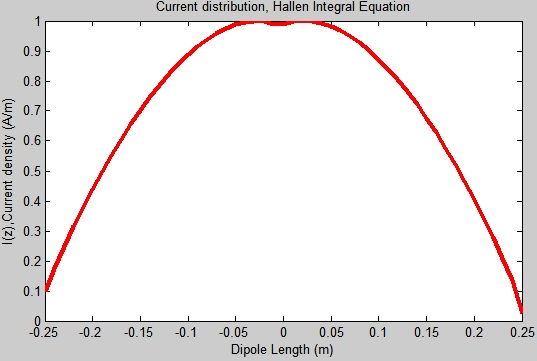
\includegraphics[scale=0.5]{image4.jpg}
\caption{Hallen's Integral Equation; Current distribution on the wire antenna with f=300MHz, L=$\frac{\lambda }{2}$, 2a=$\frac{\lambda }{500}$ and N=51}
\end{figure}
\begin{figure}[here!]
\centering
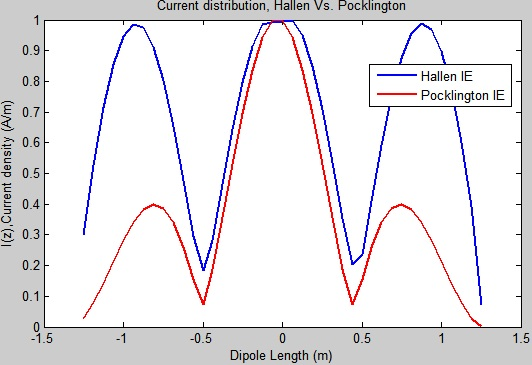
\includegraphics[scale=0.5]{image5.jpg}
\caption{Current distribution on the wire antenna; Pocklington's vs Hallen's with f=500MHz, L=$1.5 \lambda$, 2a=$\frac{\lambda }{200}$ and N=41}
\end{figure}
Figure 4 Shows the surface current distribution on the linear dipole antenna using Hallen's integral equation for point matching MoM. The frequency of operation is 300 Mhz, length of dipole is $\frac{\lambda }{2}$, diameter of wire is $\frac{\lambda }{500}$ and N=51.\\
Total simulation time is 177.259 sec. During the simulation the maximum time was consumed to manipulate symbolic variables in the MATLAB code which plays an important role in the integration. The quad function was called 2652 times with total time 6.776 ses.\\
 Figure 5 shows the comparison between surface current distribution between Pocklington's and Hallen's for frequency=500MHz, length of dipole is $ 1.5 \lambda $ and diameter of wire is $ 0.005 \lambda $ and N=41.
\section{Conclusion}
The implementation of Method of Moment using MATLAB is presented here. The Pocklington's and Hallen Integral equation is used for the analysis of linear wire antenna.The subdomain and entire domain basis function have been studied. The essential elements of Pocklington's and Hallen's IE, Basis and Testing functions, source modeling have been reviewed and implemented in MATLAB.The convergence of the solution for different source modeling have been investigated.\\
 The MoM for the wire antennas proved to be a good tool for analysis and its successful example is ``4NEC2x". The MoM based numerical techniques are easy to implement but the user should be careful since the solution required integral equation within the code. 
\subsection*{Appendix A:  Source Modeling}
The source modeling is an important parameter because it affect the antennas impedance characteristics \cite{gibb}.  As discussed in previous section, the Hallen's IE is restricted to delta gap excitation but Pocklington's IE can use any of the excitation model. There are two main excitation model: Delta-Gap excitation, and Magnetic Frill.\\
\textbf{1. Delta-Gap excitation:} The delta gap source treats the feed as if the electric field impressed by the feed line exists only in the gap between the antenna terminal and is zero outside, i.e. no fringing \cite{gibb}.Mathematically, 
\begin{equation}
E^i=\frac{V_o}{\Delta_z} \hat{z}
\end{equation}
where $ \Delta_z $ is the width of the gap, and $ V_o $ is generally set to unity. This is shown in Figure 6(a).\\
\begin{figure}[here!]
\centering
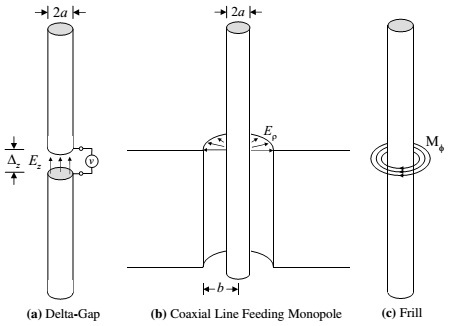
\includegraphics[scale=0.5]{source.jpg}
\caption{Thin wire source modeling \cite{gibb}}
\end{figure}
\begin{figure}[here!]
\centering
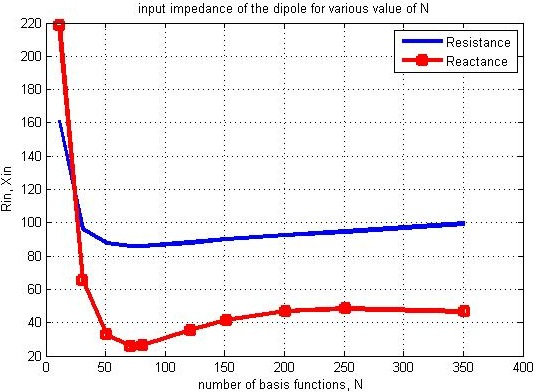
\includegraphics[scale=0.5]{delta.jpg}
\caption{Convergence of input impedance; Delta-Gap source}
\end{figure}
\begin{figure}[here!]
\centering
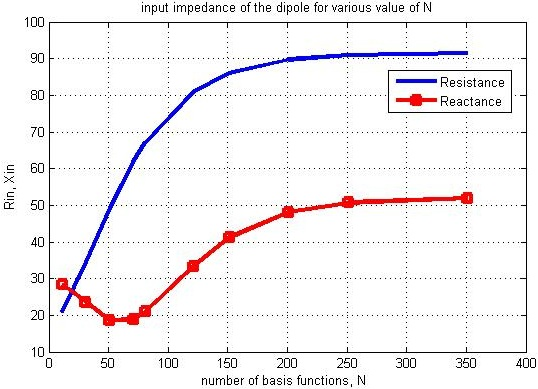
\includegraphics[scale=0.5]{frill.jpg}
\caption{Convergence of input impedance; Magnetic Frill}
\end{figure}
\textbf{2. Magnetic Frill: } Figure 6(b) shows the coaxial line feeding a monopole antenna over an infinite ground plane. If the field inside the aperture is pure TEM, then using method of image we can replace the aperture and ground plane with magnetic frill; as shown in Figure 6(c).The impressed electric field for magnetic frill can be given as,
\begin{equation}
E^i=\frac{1}{2log(b/a)} \left ( \frac{e^{-jkR_1}}{R_1}-\frac{e^{-jkR_2}}{R_2} \right )
\end{equation}
\textbf{MATLAB code for source modeling: } The MATLAB code for Delta excitation is:
\begin{lstlisting}
	V(Is) = -i*w*ep0*Vo/h;
	% ep0 is Permittivity of free space
	% w is the angular frequency
\end{lstlisting}
The MATLAB code for Magnetic frill is:
\begin{lstlisting}
	V=transpose(-i*w*ep0*Vo/2/log(2.3)...
	    *(exp(-i*k*r1)./r1-exp(-i*k*r2)./r2));
	% k is wave number
\end{lstlisting}
Figure 7 shows the Convergence of input impedance in case of delta-gap source model. The delta-gap source converge faster, and for our problem it converge when N=51. Similarly, Figure 8 shows the Convergence of input impedance in case of magnetic frill source model . The convergence of the magnetic frill was observed N>90  The Pocklington's IE is used for the analysis. For the analysis, $ \lambda =2 meter $, $ a=0.002 \lambda $ and $ L= 0.5 \lambda $ is used. 
\begin{figure}[here!]
\centering
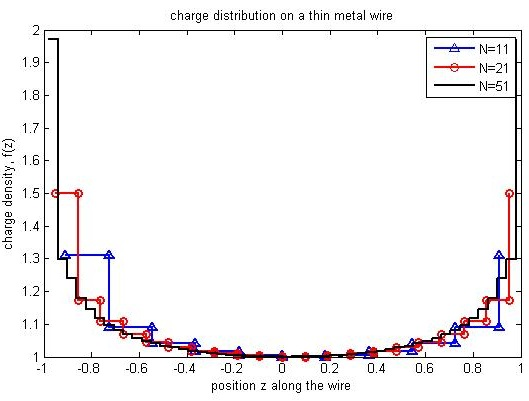
\includegraphics[scale=0.5]{subd.jpg}
\caption{Surface current on wire antennas for N=11,21,51; Subdomain Basis Function }
\end{figure}
\subsection*{Appendix B:  Basis and Weighting Function}
\textbf{Basis Functions or Expansion Function: } There are two main class of basis function. These are subdomain basis functions and entire domain \cite{garg}.\\ 
\textit{Subdomain Basis Function: } The subdomain basis function take the guesswork out of the unknown distribution and very versatile in nature. In this case, the domain is discretized in equal or unequal segment size. Every subdomain is spanned by subdomain function. The subdomain basis functions are nonzero over the subdomain ( or segment) and zero outside, and in this way it model the unknown distribution function. The example of subdomain basis function are Pulse basis function, Triangular basis function, spline basis function etc.\\
\textit{Entire Domain Basis Function: }As name suggests, the entire domain basis functions are defined over the entire domain (the range of space variable over which the problem is defined).\\
\textbf{Weighting Functions or Testing Functions: } In the Method of Moment, point matching and Galerkin's method id most common ways to solve IE problems. In the point matching method, Dirac pulses are used as weighting functions. Mathematically, 
\begin{equation}
w_{m}(z)=\delta (z-z_m)
\end{equation}
In the Galerkin's method, weighting functions are identical with the basis functions, i.e.
\begin{equation}
w_{m}(z)=f_{m}(z)
\end{equation}
Figure 9 shows the surface charge on the wire antenna for different value of N. The subdomain basis function is used for the solution.\\
Figure 10 shows the surface charge on the wire antenna for different value of N. The entire domain basis function is used for the solution. 
\begin{figure}[here!]
\centering
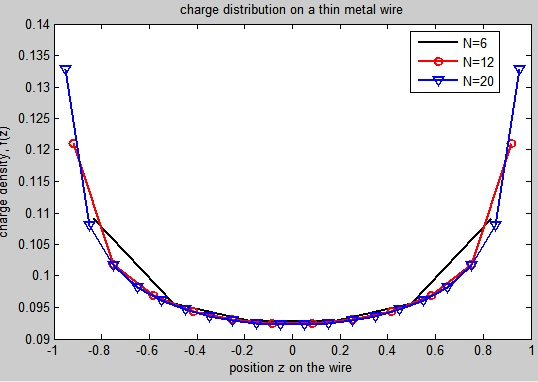
\includegraphics[scale=0.5]{entire.jpg}
\caption{Surface current on wire antennas for N=6,12,20; Entire Basis Function }
\end{figure}
\begin{thebibliography}{99}
\section*{\large{References}}
\bibitem{sadiku}
Matthew N. O. Sadiku, "Numerical Techniques in Electromagnetics with MATLAB", Third Edition, CRC Press\\
\bibitem{garg}
Ramesh Garg, "Analytical and Computational Methods in Electromagnetics", Artech House, Inc., 2008\\
\bibitem{harri}
R. F. Harrington, "Fields Computation by Moment Methods", Wiely IEEE Press, 1993\\
\bibitem{bala}
Constantine A. Balanis, "Advanced Engineering Electromagnetics", Wiely India Pvt. Ltd., 2008\\
\bibitem{paper1}
W.D. Rawle, "The Method of Moments: A Numerical Technique for Wire Antenna Design", High Frequency Electronics, Summit Technical Media,pp. 43-47,  February 2006\\
\bibitem{matlab}
MATLAB 2013b User Manual\\
\bibitem{gibb}
Walton C. Gibson, "The Method of Moments in Electromagnetics", Chapman and Hall / CRC, 2008\\
\bibitem{class}
Computational Electromagnetics, Lecture Notes, EE640, IIT Kanpur.\\
\end{thebibliography}
\end{document}

